\chapter{Introduction}

We all rely on messaging applications like WhatsApp, Facebook Messenger, Signal, etc.\ in our daily lives and take it for granted that our messages will be transmitted securely, for some definition of ``secure''. A common security feature expected from the protocol employed in a messaging application and known also to the general public is end-to-end encryption, i.e.\ that only the end users of a messaging session can read the messages being sent and the service provider or any party with access to the communication channel learns nothing of their contents. Another straightforward feature is that the protocol should work in an asynchronous setting: we would like to send messages even when the recipient is offline, and we expect them to receive the messsage once they come online. For this we must rely on a delivery service to store and deliver the messages. Of course also this delivery service should learn nothing about the contents of the messages.

There are two more advanced security features expected from messaging protocols today, both related to security in case a user is compromised:
\begin{itemize}
	\item forward secrecy (FS): the compromise should not reveal the contents of old messages
	\item post-compromise security (PCS): after the user recovers from the compromise, new messages are secure once again
\end{itemize}
As a user may well not know that they have been compromised, ensuring PCS requires regularly updating the key material used for encryption (in a way that the information leaked in a compromise \emph{before} the update does not suffice to compute encryption keys used \emph{after} the update). The more often the key material is updated, the stronger the level of PCS that is achieved. Thus, updating the key material should be an efficient operation.

For messaging between two users, the Double Ratchet protocol \cite{double-ratchet}, the main component of the so-called Signal Protocol, is a widely adopted solution used by major messaging applications such as Signal, WhatsApp, Facebook Messenger and more. It is well studied and achieves all of the above security guarantees \cite{double-ratchet-analysis}. For messaging in a group of more than two users, a straightforward solution is to maintain 1:1 communication channels using the Double Ratchet protocol between every pair of users and send messages to the group by sending them to every member individually. This achieves very strong security guarantees, but requires a number of encryption operations linear in the group size to send a message.

Another common solution is to use sender keys \cite{sender-keys}: every user creates a symmetric key, their \emph{sender key}, and distributes this sender key to every other user using 1:1 channels as before. A user sending a message then derives a symmetric encryption key for the message from their sender key, while continually updating their sender key (with each sent message) to provide FS. However, achieving PCS is costly: if a user is compromised, the sender keys of all users are leaked and recovering from the compromise requires each user to send a new sender key to every other user over the respective 1:1 channels, resulting in a number of operations linear in the group size per user and a quadratic number of operations in total. Moreover, dynamic group membership introduces additional complexity:
\begin{itemize}
	\item adding a new member involves the new member sharing their sender key with all other group members
	\item removing a member requires distributing new sender keys in the group, just like recovering from a compromise
\end{itemize}
The Messaging Layer Security (MLS) protocol, recently standardized in \cite{rfc9420}, proposes a solution for group messaging with better efficiency and the same strong security guarantees as for the two-party case. Updating key material and adding or removing members can be achieved with a logarithmic number of operations (although the complexity may still degrade to linear in certain scenarios). At the core of MLS is a fairly recent primitive called a \emph{continuous group key agreement} (CGKA) scheme \cite{rtreekem} (this primitive was introduced only \emph{after} the first draft of the MLS protocol). In essence, a CGKA scheme enables a group of users to agree on a \emph{group key}, which they can then use to derive symmetric message encryption keys. This key must be indistinguishable from a random key for anyone outside the group eavesdropping on all communication. However, a CGKA scheme must also achieve FS and PCS, and support dynamic group membership. Hence, it must provide mechanisms for members to update their key material, add new users to the group and remove members from the group. Moreover, the scheme must work in the asynchronous setting with an untrusted service to deliver protocol messages.

The CGKA scheme used in the MLS protocol is called TreeKEM (initially proposed in \cite{treekem}) and the majority of the literature on MLS is dedicated to analyzing TreeKEM or proposing better CGKA schemes as in \cite{ttkem,rtreekem,insider-security,modular-group-messaging}. The TreeKEM protocol has undergone multiple changes since its inception. In this work we refer to the version documented in RFC 9420. TreeKEM, as adopted from its predecessors, maintains a binary tree where every node in the tree has some associated secrets, every member of the group is associated with a leaf and the group key is derived from the root of the tree. Every member can compute the group key from their view of the tree. The group key can be updated and members added/removed with a number of operations logarithmic in the group size.

Given that the vision for the MLS protocol is for it to become the new standard for messaging protocols and that it has support from several large companies \cite{google-mls,mls-support}, it has the potential to be used by a huge number of users. Thus, understanding the security of MLS and hence also of TreeKEM is of great importance. This means having formal security guarantees about the security provided by TreeKEM (based on appropriate hardness assumptions). The first important step in this direction was the conception of the CGKA primitive and the accompanying definitions of security introduced in different works (for example \cite{rtreekem, ttkem}). Such definitions clarify what kind of adversaries we can provide security against and thus what kind of security one should expect from the scheme when using it in practice. Moreover, proofs of (reasonably tight) security under these definitions show what level of security we should expect from the scheme and serve as a guide to implementors on what values to choose for the security parameter. Proofs also provide strong justification that there are no flaws in the overall design of the scheme.

One choice that can be made when defining the security of a CGKA scheme is whether the adversary is modeled as \emph{selective} or \emph{adaptive}. In the former case, the adversary must provide all the interactions it will have with the protocol and when it will attempt to break the scheme at the beginning of the security game, while in the latter case the adversary can make its decisions based on responses from previous interactions. Clearly, the adaptive setting is much closer to how an attack would unfold in practice, so it is desirable to prove security against adaptive adversaries. However, achieving this without too much of a blow-up in the security loss is a challenge since one often resorts to guessing actions performed by the adversary.

The Generalized Selective Decryption (GSD) security game \cite{gsd} was introduced precisely to analyze adaptive security for protocols based on a graph-like structure (as is the case with TreeKEM). It was initially defined for the private-key setting and later adapted to the public-key setting in \cite{ttkem}. The work in \cite{ttkem} proved a polynomial bound for the adaptive security of the public-key GSD game in the so-called Random Oracle Model (ROM) for an arbitrary IND-CPA secure public-key encryption scheme. This result implies a polynomial bound for the adaptive security of TreeKEM as a CGKA scheme as outlined in \cite[Theorem 4]{ttkem} and subsequently proved in more detail in \cite[Theorem 12]{modular-group-messaging}.

In this work, we formally prove the adaptive security of a specific public-key encryption scheme, the DHIES scheme, in a modified version of the public-key GSD game, adapted to better model TreeKEM, in the ROM. Focusing on the DHIES scheme allows us to achieve a tighter bound than the one in \cite{ttkem}. Moreover, we define the syntax and security of propose and commit CGKA schemes, provide a high-level description of how the TreeKEM protocol can be instantiated with our definitions and state a result in the ROM relating the security of a public-key encryption scheme in our modified GSD game with the security of TreeKEM as a CGKA when instantiated with this public-key encryption scheme.

\section{Contributions}

We present the following main contributions:
\begin{itemize}
	\item A simple definition of an adaptation of the public-key GSD game better suited to model TreeKEM.
	\item A simple and detailed proof of (adaptive) security of the DHIES scheme with respect to our GSD definition. We achieve a tighter bound than the one proven so far.
	\item Simple and clear definitions of the syntax and security of propose and commit CGKA schemes. We explain our definition in detail and briefly discuss the correctness of CGKA schemes.
	\item A high-level description of the TreeKEM protocol and how it can be instantiated with respect to our CGKA definition. Finally, we state a result relating the security of our GSD game and the security of TreeKEM, and provide an outline of the proof.
\end{itemize}

\section{Technical overview}

\subsection{The GSD game}

In the GSD security game, given an encryption scheme a graph, the \emph{GSD graph}, is constructed by the challenger where every node in the graph is associated with a symmetric key in the private-key setting, or a public/private key pair in the public-key setting. The adversary can then request encryptions of a node's (secret) key under the (public) key of another node. In the public-key setting, such an \emph{encryption query} also reveals the node's public key. This creates an \emph{encryption edge} in the graph, directed from the node whose (public) key was used for encryption to the node whose key was encrypted. The adversary can also corrupt any node, which reveals its (secret) key and allows the adversary to compute the (secret) key of any other node reachable from the corrupted node in the graph by performing decryptions along the path to the other node. At the end of the game the adversary chooses a node to be challenged on, the \emph{challenge node}. A coin is then tossed and the adversary is given either the (secret) key of the challenge node or a uniformly random (secret) key and it must guess which scenario it is in. The possible choices for the challenge node must of course be restricted to nodes whose keys were not compromised through a corruption, meaning that the challenge node should never be reachable from a corrupted node in the graph. Further restrictions are also necessary which we do not go into here. Figure~\ref{fig:gsd-example} illustrates what an example GSD graph may look like.

\begin{figure}
	\begin{center}
		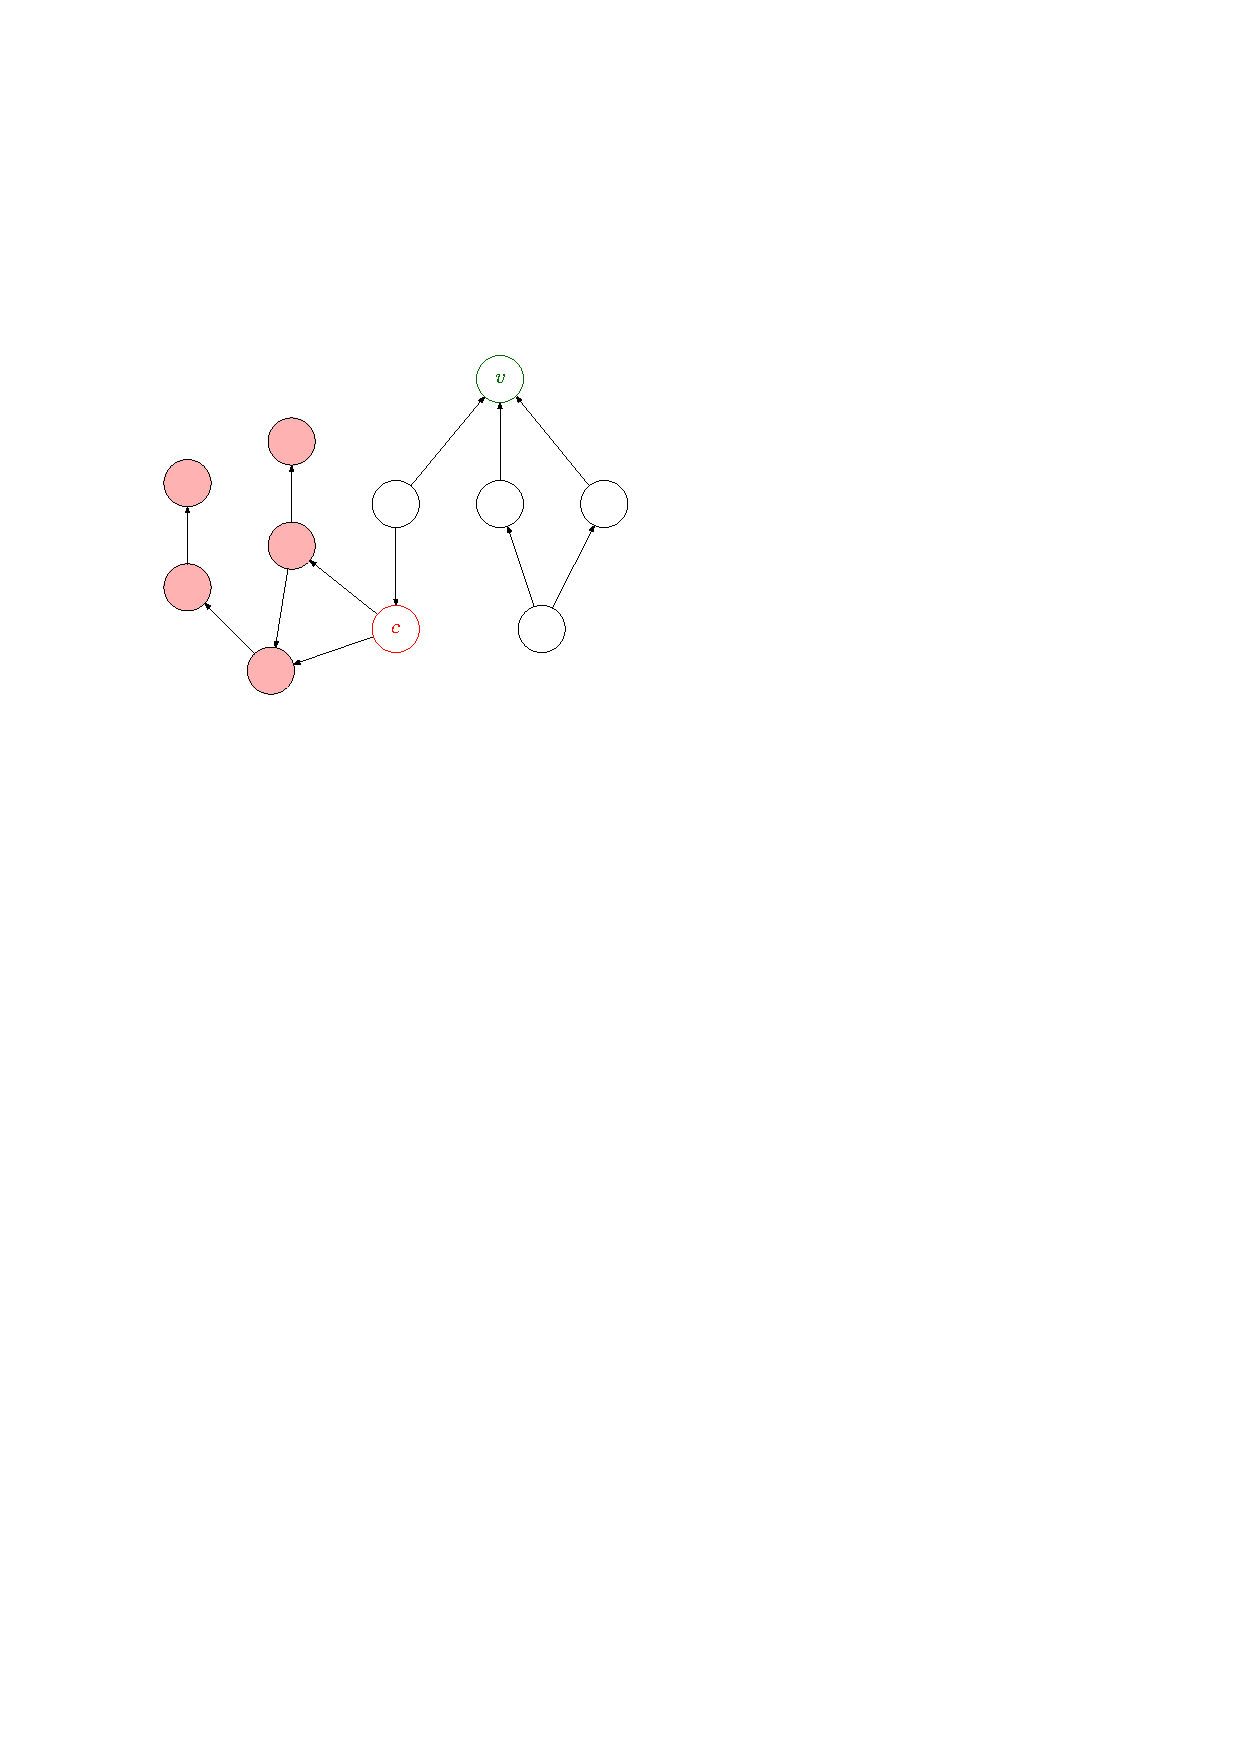
\includegraphics{figures/gsd-example}
	\end{center}
	\caption{An illustration of the GSD graph for an instance of the GSD game. The challenge node is $v$. The node $c$ was corrupted, resulting in all nodes reachable from it being compromised, as marked with red color.} \label{fig:gsd-example}
\end{figure}

\subsection{The TreeKEM protocol} \label{sec:treekem-overview}

\subsubsection{Propose and commit syntax}

As a CGKA scheme, TreeKEM must support operations for updating the key material of a group member, adding a new user and removing a member. The syntax for these operations has changed over time. In the current version of MLS, the protocol uses so-called \emph{proposals} and \emph{commits}. Whenever a user would like have their key material updated (by someone else), add a new user or remove a group member, they create a corresponding \emph{update}, \emph{add} or \emph{remove proposal}, respectively, and share this proposal with the group. Any group member can then create a \emph{commit} to apply a set of proposals, create a new group key and update their key material in the process. The commit object includes (encrypted) information such that every group member can update their view of the group and compute the new group key.

\subsubsection{TreeKEM dynamics}

As already outlined briefly, TreeKEM uses a full binary tree to model the group. Every user, associated with a leaf in the tree, maintains a synchronized view of the tree, though different users will know more about different parts of the tree. The group key is derived from the root of the tree. Every node $n$ in the tree has an associated key pair $(pk_n, sk_n)$ output by $\Pi.\gen$ where $\Pi$ is a public-key encryption scheme. All public keys are known to all users. Let the \emph{direct path} of a leaf be the path from the leaf's first parent to the root. Every user at a leaf knows the secret key of their leaf and, in the usual case, the secret keys of all nodes on their direct path, though we will see exceptions to this rule later. To illustrate the scheme and how commit operations are performed, we will consider of a group with users $A, B, \ldots, G$ and $H$, as depicted in Figure~\ref{fig:treekem-tree}. In the following, we will use these labels for the users both to refer to the users themselves and to their nodes in the tree.

\begin{figure}
	\begin{center}
		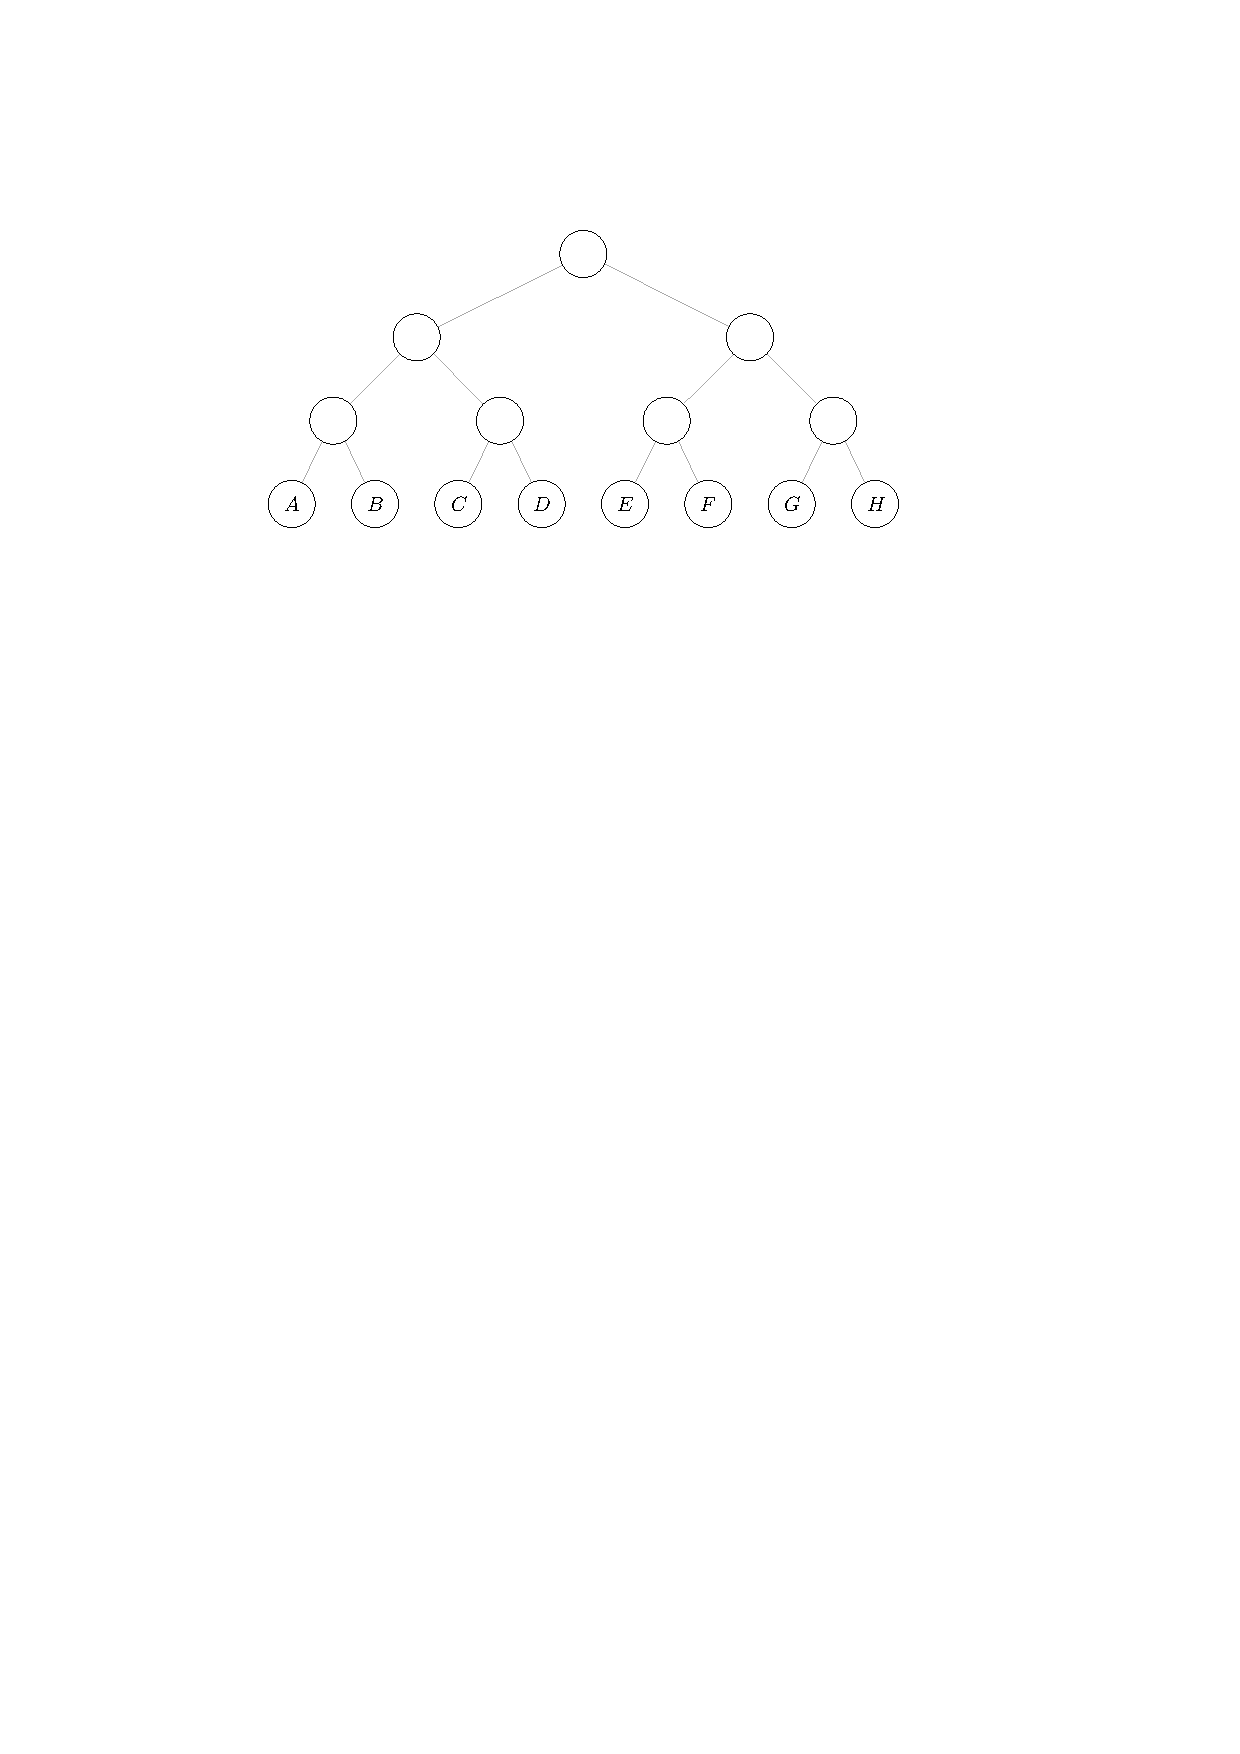
\includegraphics{figures/treekem-tree}
	\end{center}
	\caption{Illustration of a group with users 8 users in the TreeKEM protocol.}\label{fig:treekem-tree}
\end{figure}

\paragraph{Simple commits} The idea behind this tree structure is that it allows for a user creating a commit with a new group key to share the new group key with the group using only a few encryptions, while still updating all the secrets the user knew in the tree in order to recover from a possible compromise (recall that in a PC-CGKA scheme a commit also updates the committer's key material).
To illustrate how a commit is performed and how the new group key is computed, say user $A$ performs a commit. First we only consider commits without any proposals. TreeKEM specifies two hash functions $\hgen, \hdep \colon \{0, 1\}^{\rho(\eta)} \to \{0, 1\}^{\rho(\eta)}$ where $\rho(\eta)$ gives the number of bits of randomness used by $\Pi.\gen(1^\eta)$. Let $d = 3$ the depth of user $A$. $A$ will replace all the $d + 1$ nodes on their path to the root (including their leaf) with new nodes $A, p_1, \ldots, p_d$. Although it would be more accurate to say that $A$ just replaces the information stored in the original nodes, and this view makes more sense when implementing the protocol, it will become convenient later to say that $A$ creates new nodes.
The key pairs for the new nodes are sampled as follows. For the leaf node $A$, user $A$ simply samples a key pair by running $\Pi.\gen(1^\eta)$. For the remaining nodes, they first sample $s_1 \from \{0, 1\}^{\rho(\eta)}$ and compute the key pair of the first parent $p_1$ as $\Pi.\gen(1^\eta, \hgen(s_1))$. For $i \in \{2, \ldots, d\}$ they then compute $s_i \coloneqq \hdep(s_{i - 1})$ and set the key pair of $p_i$ to be $\Pi.\gen(1^\eta, \hgen(s_i))$. The new group key is $k \coloneqq \hdep(s_{d})$.

User $A$ only needs to share (encryptions of) the seeds $s_i$ for the other users to update their view of the tree and compute the new group key:
\begin{itemize}
	\item To share the group key with user $B$, $A$ computes the ciphertext $c_1 \coloneqq \Pi.\enc_{pk_B}(s_1)$. $B$ can then compute the seed $s_1$, then use that to compute the seeds $s_2, \ldots, s_d$, the key pairs of all new nodes on their path to the root and the group key $k$.
	\item To share the new group key with users $C$ and $D$, $A$ computes the ciphertext $c_2 \coloneqq \Pi.\enc_{pk_X}(s_2)$, where $X$ is the parent of the nodes $C$ and $D$. Both $C$ and $D$ know the secret key $sk_X$ of their parent and can decrypt $c_2$.
	\item To share the new group key with users $E, F, G$ and $H$, $A$ computes the ciphertext $c_3 \coloneqq \Pi.\enc_{pk_Y}(s_3)$, where $Y$ is the right child of the root node. Again, all users under $Y$ know $sk_Y$ and can thus decrypt $c_3$.
\end{itemize}
The commit $c$ that $A$ shares with all users includes the ciphertexts $c_1, c_2$ and $c_3$ and the public keys of all new nodes. Figure~\ref{fig:treekem-simple-update} illustrates the commit performed by $A$.

\begin{figure}
	\begin{center}
		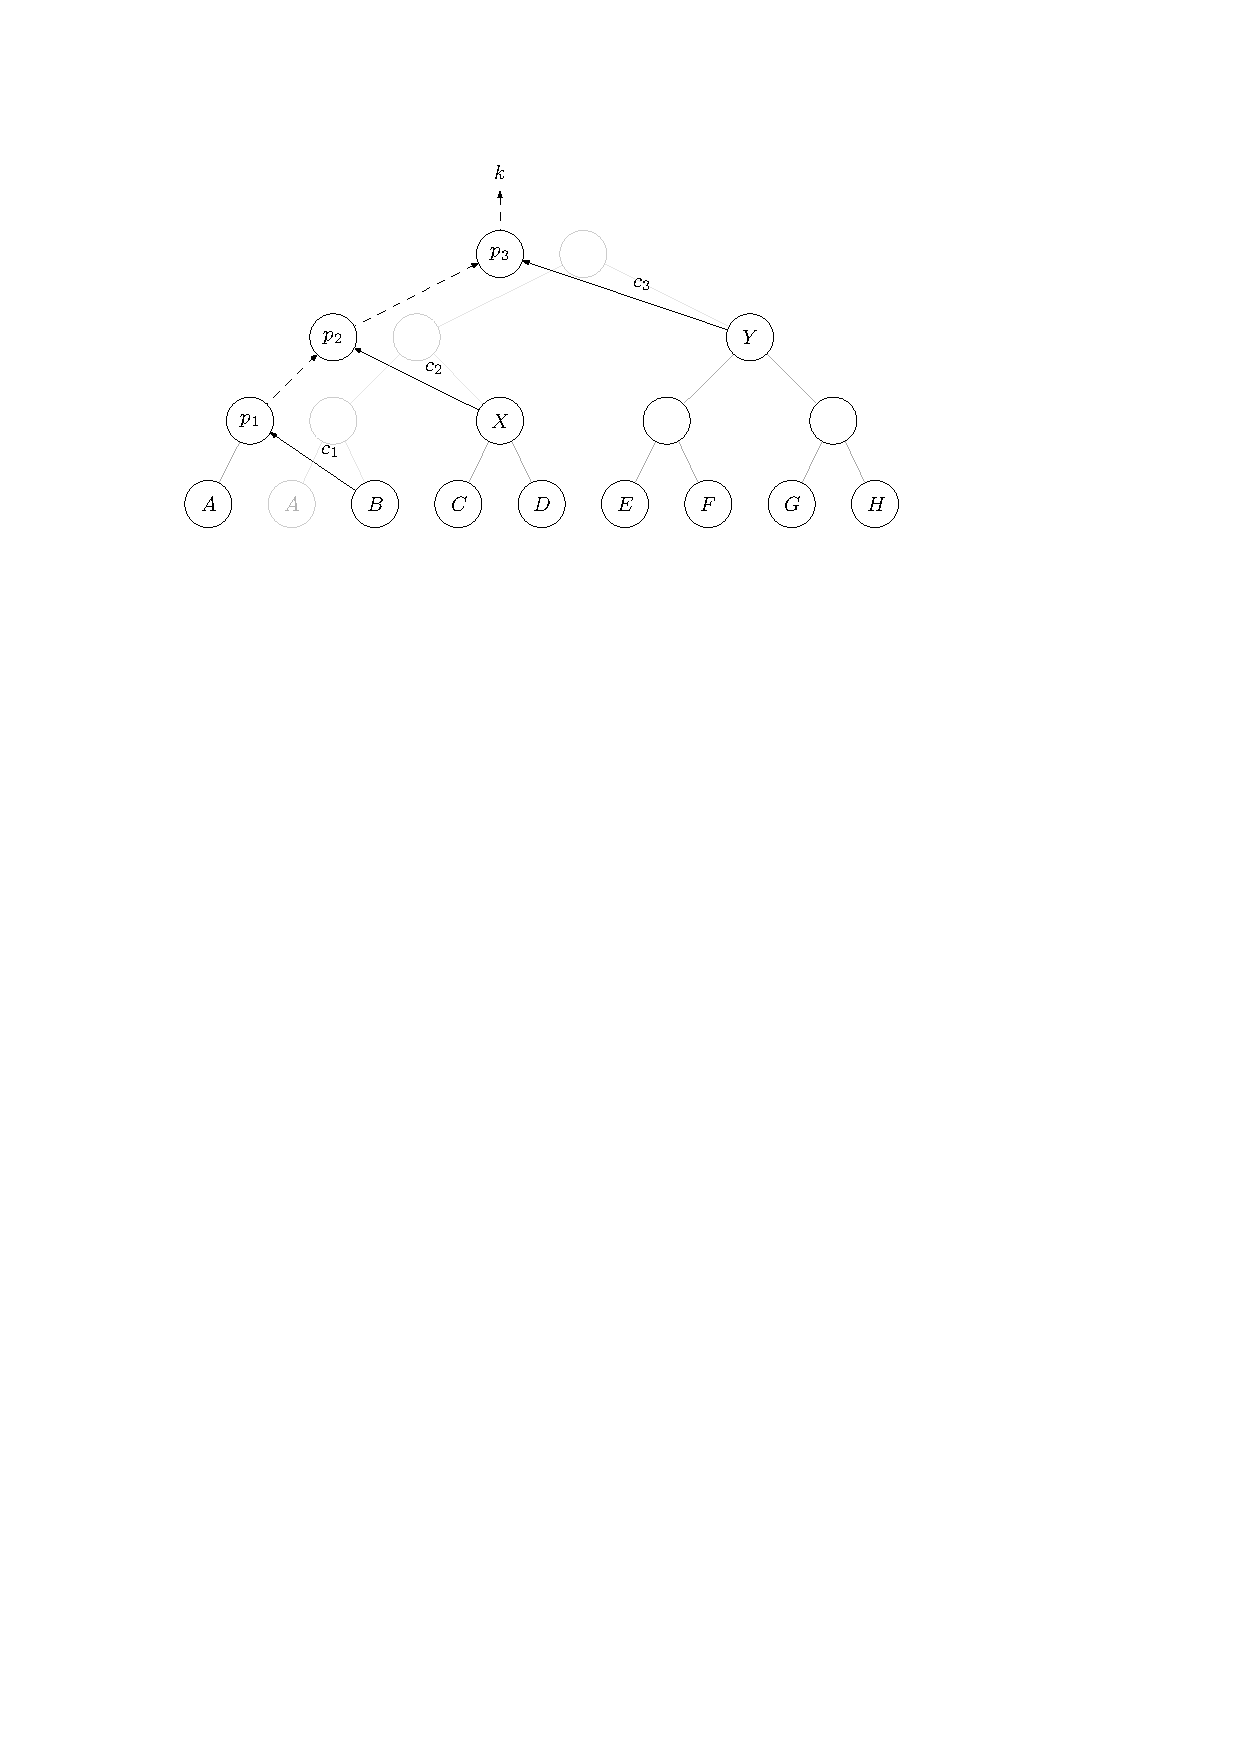
\includegraphics{figures/treekem-simple-update}
	\end{center}
	\caption{The commit by user $A$ described in the text. Dashed directed edges illustrate the fact that the target is related to the source via the hash function \question{Should I call this a PRF instead?} $\hdep$. The solid directed edges illustrate the fact that the seed of the target node is encrypted to the public key of the source node.}\label{fig:treekem-simple-update}
\end{figure}

The nodes $B, X$ and $Y$ form the \emph{copath} of $A$: the copath of a node consists of the sibling of each node on the node's path to the root, excluding the root itself. In the ideal case as above, a node performing a commit only has to compute one encryption for each node on its copath, i.e. logarithmically many encryptions in the total number of users.

\paragraph{Remove and update proposals} Things look a bit different if the commit contains a remove proposal. Say user $A$ creates a commit that contains a remove proposal for user $E$. We could just let $A$ replace the nodes on $E$'s direct path $E$ and not encrypt anything for $E$. However, if $A$ were compromised while replacing $E$'s direct path and performed another commit to update their key material after the compromise, the information leaked in the compromise could still be used to compute the new group key, as it includes the secret keys of the nodes on $E$'s direct path.
Instead, $E$'s leaf and all nodes on $E$'s direct path are replaced by \emph{blank} nodes: nodes with no associated key pair. Now $A$ has to encrypt the secret $s_3$ directly to $F$ and to the parent node of $G$ and $H$ in the commit removing user $E$. See Figure~\ref{fig:treekem-remove}. A blank leaf node can be populated with a new user. A blank node that is not a leaf will be replaced by a non-blank node once some user in the node's subtree performs a commit. Blank nodes are also useful to represent the nodes of a subtree with no users.

\begin{figure}
	\begin{center}
		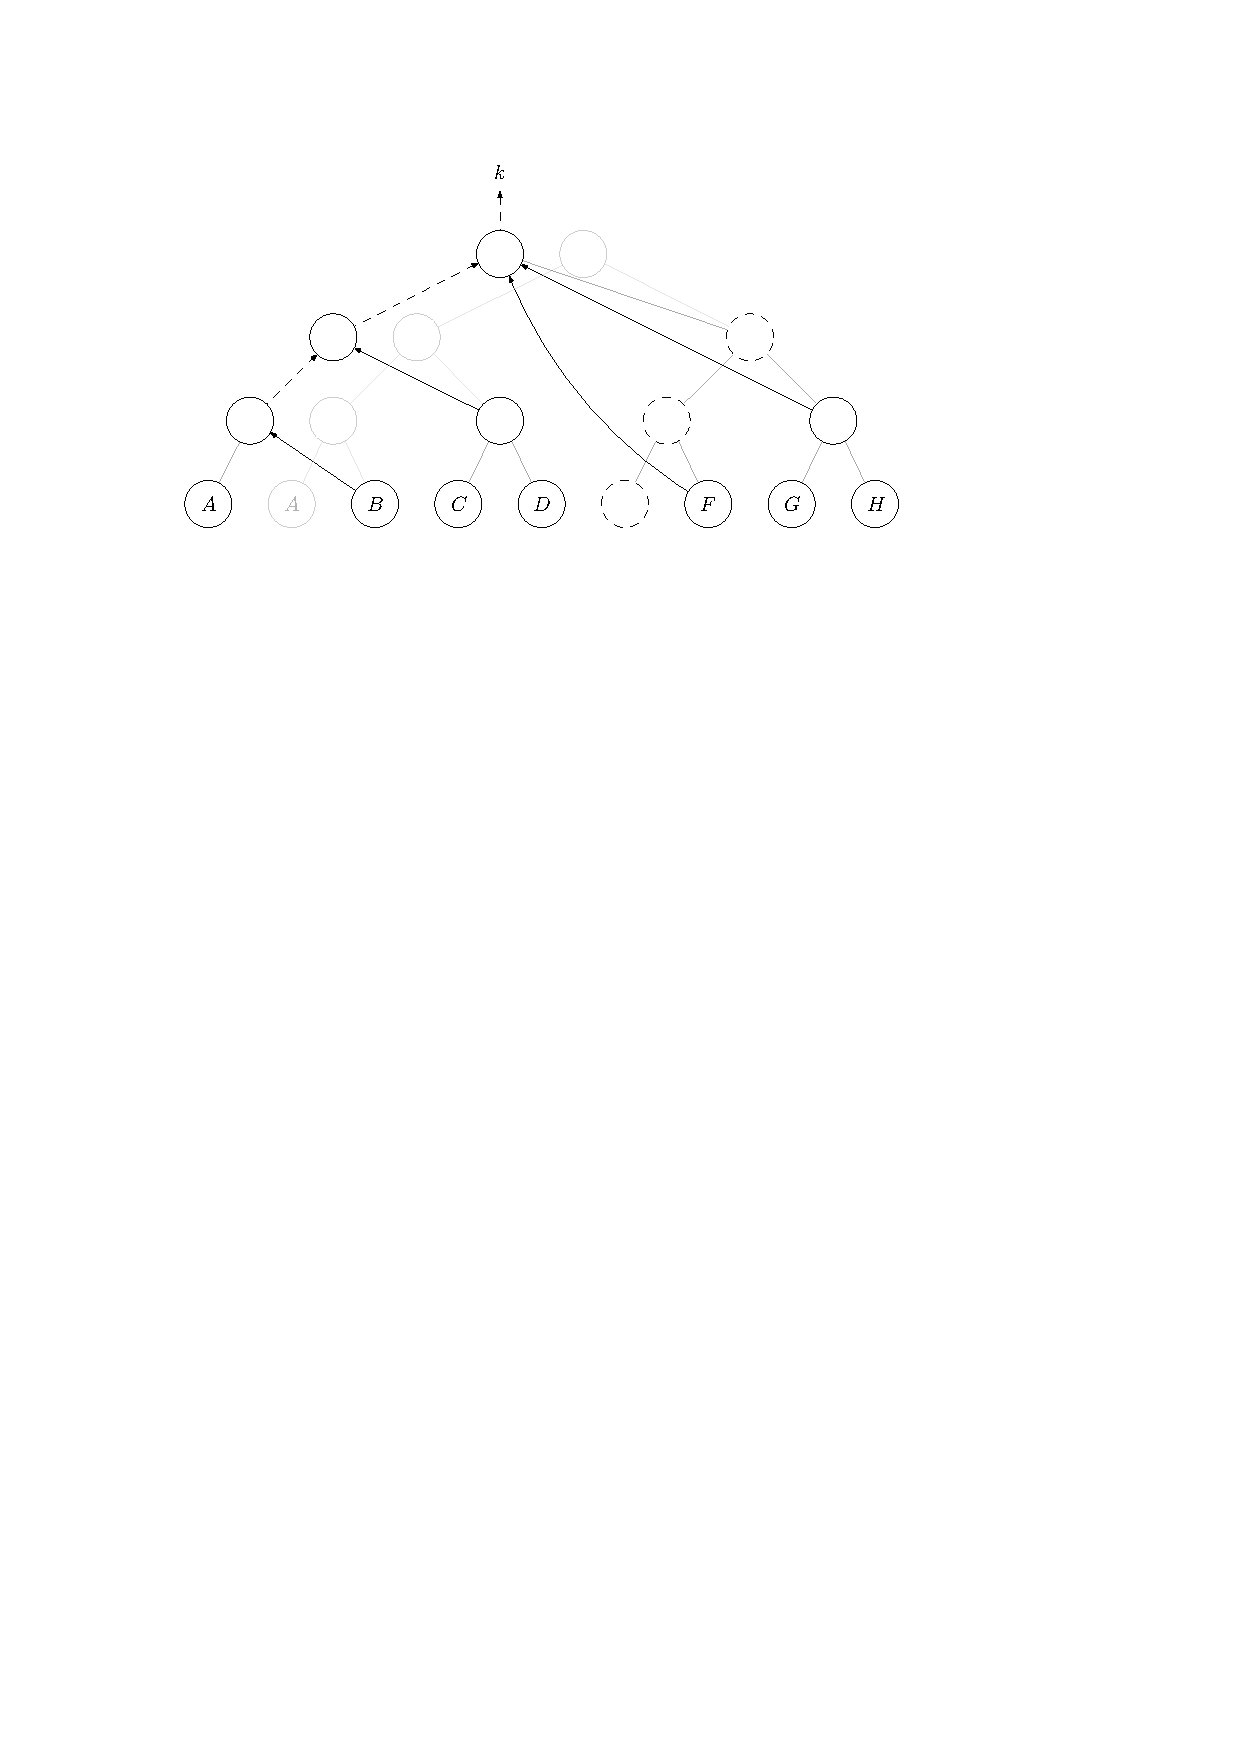
\includegraphics{figures/treekem-remove}
	\end{center}
	\caption{The commit by user $A$ removing user $E$ described in the text. Nodes with a dashed border represent the (new) blank nodes.}\label{fig:treekem-remove}
\end{figure}

Creating a commit with an update proposal for user a $u$ is analogous. The update proposal simply contains the public key of user $u$'s new leaf, while $u$ stored the corresponding secret key locally when creating the proposal. Because we don't want the committer to know the secret keys along $u$'s direct path, we must again replace these nodes with blank ones and encrypt to the non-blank nodes below directly.

\paragraph{Add proposals} Adding a user introduces one new but similar complication. Consider the same group as in Figure~\ref{fig:treekem-tree}, but with the leaf of user $H$ blank. Now say user $A$ would like to add user $H$ to the group. Although we would want $H$ to know all secret keys on their direct path, $A$ can only provide the secrets of their lowest common ancestor, which is the root node in this case.
In such a situation where a non-blank node $n$ has a leaf $l$ below it where $l$ does not know $n$'s secret key, we say that $l$ is \emph{unmerged} relative to $n$. Every non-blank, non-leaf node stores its list of unmerged leaves and whenever one encrypts to a node, one should also encrypt to all its unmerged leaves. A user's leaf becomes ``merged'' as the nodes on their direct path are replaced and they are provided the seeds to compute the secret keys of the new nodes.
Note that for any non-leaf node $n$, any one of its descendants $d$ and any unmerged leaf of $n$ that is a descendant of $d$, this leaf must also be an unmerged leaf of $d$: every commit that replaces $d$ also replaces the node $n$ and if a user at a leaf learns the secret key of the new node for $d$ through its seed, they also learn the seed of and therefore the secret key of the new node for $n$. Figure~\ref{fig:treekem-add} shows a commit by user $A$ adding $H$, followed by another commit by user $E$.

\begin{figure}
	\centering
	\begin{subfigure}[b]{\textwidth}
		\centering
		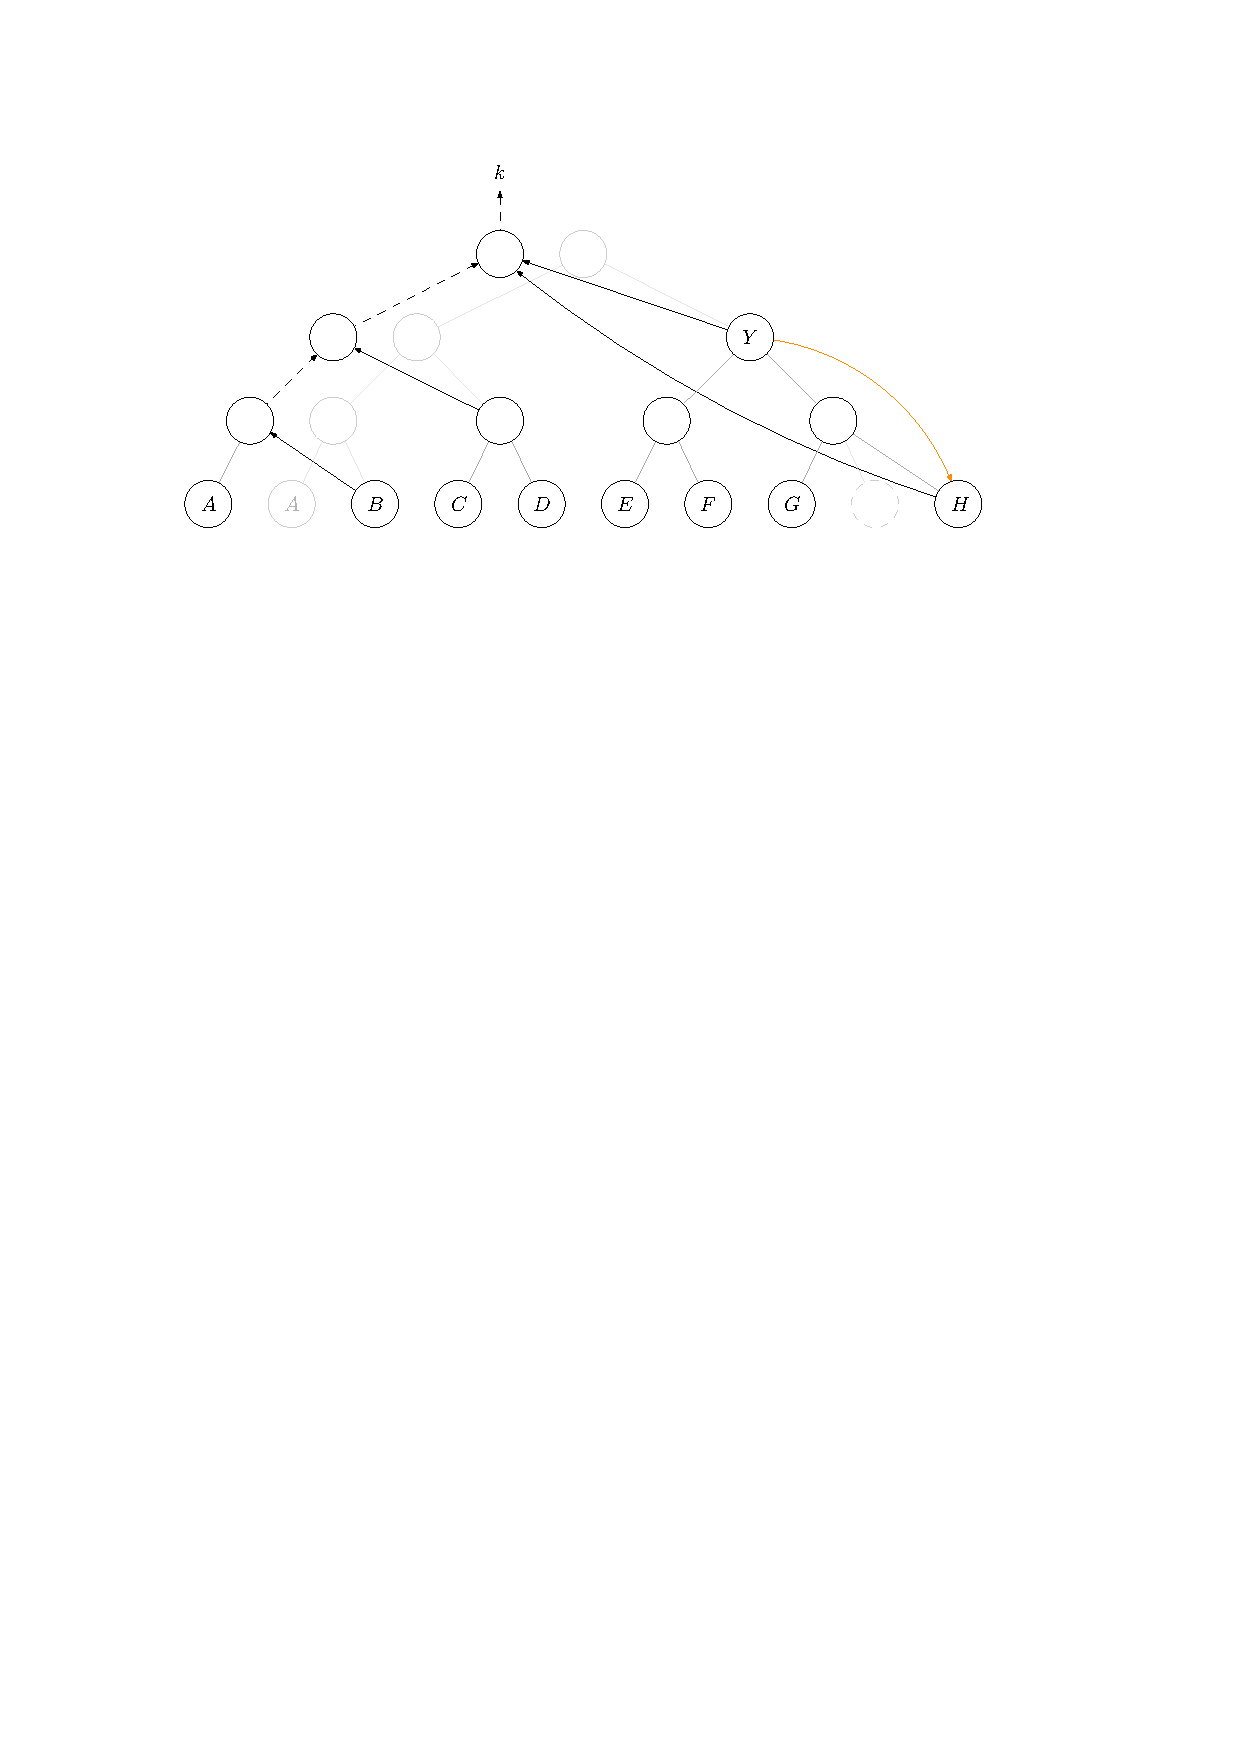
\includegraphics[width=\textwidth]{figures/treekem-add-1}
		\caption{User $A$ adds user $H$. As a small detail: the encryption for user $H$ is computed using $H$'s init key as instead of the public key of their leaf.}
		\label{fig:treekem-A-add-H}
	\end{subfigure}
	\begin{subfigure}[b]{\textwidth}
		\centering
		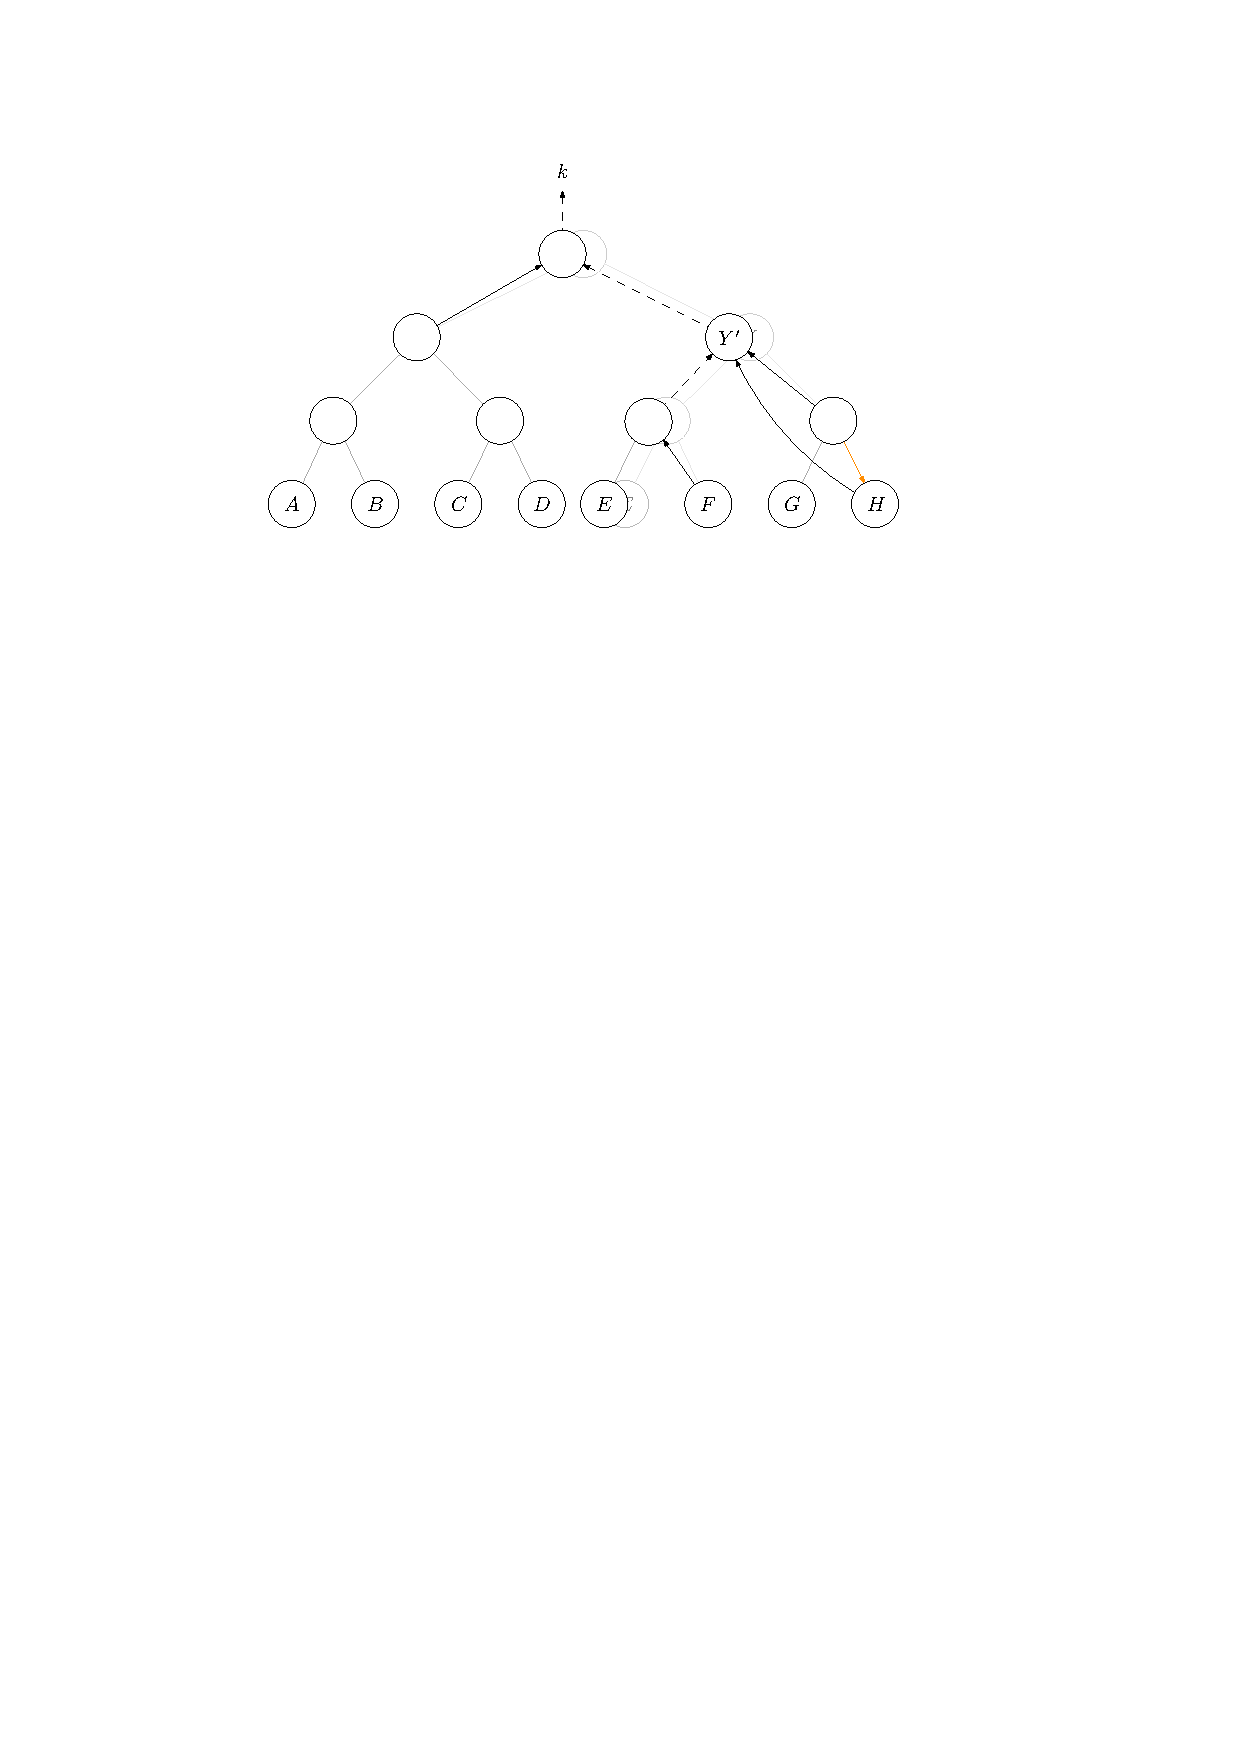
\includegraphics[width=\textwidth]{figures/treekem-add-2}
		\caption{Commit by user $E$. $H$ is now ``merged'' relative to node $Y'$.}
	\end{subfigure}
	\caption{A commit adding user $H$ and another commit by a user $E$ as described in the text. Orange edges illustrate the fact that the target leaf is unmerged relative to the source node. In \subref{fig:treekem-A-add-H}, $H$ is also unmerged relative to $Y$'s right child, but this information is redundant as it follows from $H$ being unmerged relative to $Y$.}
	\label{fig:treekem-add}
\end{figure}

\paragraph{Resolution} We have now seen that when performing a commit, one must pay attention to blank nodes and unmerged leaves when providing encryptions. Instead of only providing encryptions for each node on the copath as in the ideal case, in the general case for each node $n$ on the copath one must provide an encryption for every node in the \emph{resolution} of $n$. The resolution of a non-blank node is the node itself and the set of all its unmerged leaves. The resolution of a blank leaf is the empty set and the resolution of a blank, non-leaf node is the union of the resolutions of its two children.

\paragraph{Key packages and welcome messages} To encrypt to an existing group member it is clear that we can just use the public key in their leaf. But how do we encrypt to a new user? Before a user joins any group, they publish a \emph{key package}: this contains (among other things) the public key, their so-called \emph{init key}, to be used to encrypt information to the user when they join the group and the public key that should be associated with the user's leaf. The key package is included (or referenced) in the add proposal for the new user. Along with the seed of the committer's and the new user's lowest common ancestor in the tree, the new user must also be given the (public) state of the tree. This information is provided to the new user, encrypted with their init key, by the committer in a \emph{welcome message}.
